\documentclass{beamer}

\mode<presentation> {
  \usetheme{Madrid}
  \setbeamercovered{transparent}
}

\usepackage[spanish]{babel}
\usepackage[utf8]{inputenc}

\usepackage{amsmath}
\usepackage{graphicx}
\usepackage{fancyvrb}

%Definimos nuestra ruta para las imagenes
%Absoluto
%\graphicspath{ {/home/user/images/} }
%Relativo (recomendado) -> seg�n
%https://es.sharelatex.com/learn/Inserting_Images#La_ruta_a_la_carpeta_de_im.C3.A1genes
\graphicspath{ {../../media/} }


\title{\textbf{Introducci�n a las herramientas para el desarrollo con FPGAs}}

\author{Horacio Arnaldi}

\date{} % Colocar aqu� la fecha exacta

\subject{Generaci�n de presentaciones}

%\pgfdeclareimage[height=0.8cm]{university-logo}{logo}
\logo{
\includegraphics[width=8mm]{../../media/logos/cnea_logo}}
\logo{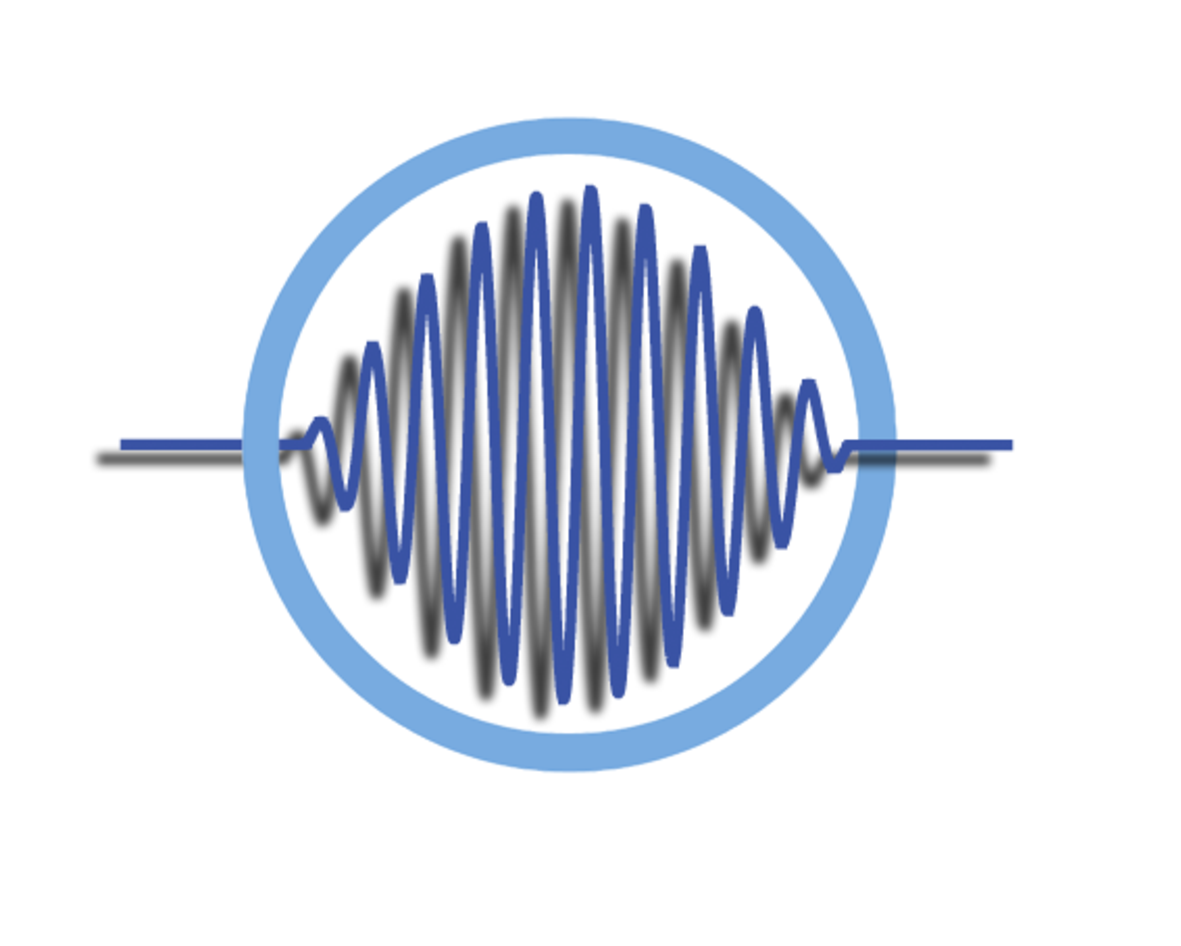
\includegraphics[width=8mm]{../../media/logos/LabDPR_logo}}
\logo{
\includegraphics[width=8mm]{../../media/logos/balseiro_logo}}



%\beamerdefaultoverlayspecification{<+->}

\begin{document}

\begin{frame}
  \titlepage
\end{frame}


\begin{frame}
  \frametitle{Contenido}
  \tableofcontents[pausesections]
\end{frame}


\section{M�quinas de estados finitos \(FSM\)}

\subsection{M�quinas de estados Algor�tmicas \(ASM\)}

\begin{frame}
    \frametitle{T�tulo de la primera diapositiva}
\begin{columns}
 \begin{column}{0.55\textwidth}
\begin{block}{Resultados}
    \begin{itemize}[<+->]
      \item  Primer item
      \item  Segundo item
      \item  Tercer item
    \end{itemize}
    \begin{enumerate}[<+-| alert@+>]
      \item  Primer item
      \item  Segundo item
      \item  Tercer item
    \end{enumerate}
\end{block}
 \end{column} \ \
 \begin{column}{0.40\textwidth}
      \only<4>{\includegraphics[width=0.8\textwidth]{../media/knuth.jpg}}
      \only<5>{\includegraphics[width=0.9\textwidth]{../media/forges.jpg}}
      \only<6>{\includegraphics[width=0.9\textwidth]{../media/kill-bill-2.jpg}}
 \end{column}
\end{columns}
\end{frame}


\subsection{Segunda subsecci�n}

\begin{frame}
    \frametitle{T�tulo de la segunda diapositiva}
\begin{block}{}
Escribimos una peque�a f�rmula
\end{block}

\begin{block}{F�rmula}
\begin{equation*}
\onslide<2->{V(x) = } \onslide<3->{\color<3>[rgb]{1,0,0} A\int_0^\infty\frac{dr}{r} +}
\onslide<4->{\color<4>[rgb]{0,1,0} B\int_0^\infty\frac{dr}{r^2} +}
\onslide<5->{\color<5>[rgb]{0,0,1} C\int_0^\infty\left(\frac{1}{r^6} - \frac{1}{r^{12}}\right)dx}
\end{equation*}
\end{block}
\end{frame}

\begin{frame}
    \frametitle{T�tulo de la tercera diapositiva}
\begin{block}{}
Ahora mostramos la f�rmula de forma un poco diferente
\end{block}

\begin{block}{F�rmula}
\begin{equation*}
V(x) =  {\color<2>[rgb]{1,0,0} A\int_0^\infty\frac{dr}{r}} +
{\color<3>[rgb]{1,0,0} B\int_0^\infty\frac{dr}{r^2}} +
{\color<4>[rgb]{1,0,0} C\int_0^\infty\left(\frac{1}{r^6} - \frac{1}{r^{12}}\right)dx}
\end{equation*}
\end{block}
\end{frame}

\begin{frame}
    \frametitle{T�tulo de la tercera diapositiva}
\begin{block}{}
Otra forma un poco m�s compleja:
\end{block}
\begin{block}{Ecuaci�n}
$\displaystyle
V(x) = \onslide<2->{\color<2>[rgb]{1,0,0} A\int_0^\infty\frac{dr}{r} +}
\onslide<3->{\color<3>[rgb]{0,1,0} B\int_0^\infty\frac{dr}{r^2} +}
\onslide<4->{\color<4>[rgb]{0,0,1} C\int_0^\infty\left(\frac{1}{r^6} - \frac{1}{r^{12}}\right)dx}$

\medskip
\hspace*{15mm} \onslide<2>{\color<2>[rgb]{1,0,0} Dipolo} \hspace{7mm}
\onslide<3>{\color<3>[rgb]{0,1,0} Coulomb} \hspace{4mm}
\onslide<4>{\color<4>[rgb]{0,0,1} Van der Waals}
\end{block}
\end{frame}

\begin{frame}[t]
    \frametitle{T�tulo de la tercera diapositiva}
\begin{block}{}
Otra forma reemplazando elementos:
\end{block}
\only<2>{\visible<2>{\begin{block}{Ecuaci�n 1}
$\displaystyle V(x) = A\int_0^\infty\frac{dr}{r} \color[rgb]{1,0,0} \longrightarrow \text{Dipolo}$
\end{block}}}%
\only<3->{\visible<3->{\begin{block}{Ecuaci�n 2}
$\displaystyle W(x) = B\int_0^\infty\frac{dr}{r^2} +
C\int_0^\infty\left(\frac{1}{r^6} - \frac{1}{r^{12}}\right)dx \only<3>{ \longrightarrow \color[rgb]{1,0,0} \text{Coulomb + WdW}}$
\end{block}}}
\only<4>{\visible<4>{\begin{block}{otro bloque}
Otras cosas...
\end{block}}}
\end{frame}

\section{Segunda secci�n}

\subsection{Primera subsecci�n de la segunda secci�n}

\begin{frame}[fragile]
\frametitle{Efectos multimedia: V�deos}
\begin{columns}
\begin{column}{5cm}
\begin{block}{}
\small
\begin{Verbatim}
\begin{block}{Una pel�cula}
\includemovie[play,repeat]%
{4cm}{3cm}{random.mpg}
\end{block}
\end{Verbatim}

\textbf{Nota:} Es esencial cargar el paquete 
\textsf{movie15} en el pre�mbulo
\end{block}
\end{column}\pause \
\begin{column}{4.2cm}
\begin{block}{Una pel�cula}
\includemovie[autoplay,repeat]%
{4cm}{3cm}{../media/random.mpg}
\end{block}
\end{column}
\end{columns}
\end{frame}

\begin{frame}[fragile]
\frametitle{Efectos multimedia: V�deos}
\begin{columns}
\begin{column}{5cm}
\begin{block}{}
\small
\begin{Verbatim}
\begin{block}{Otra pel�cula}
\includemovie[autoplay,%
controls]{5.5cm}{3.75cm}%
{budweiser.mpeg}
\end{block}
\end{Verbatim}
\end{block}
\end{column}\pause \
\begin{column}{5.7cm}
\begin{block}{Una pel�cula}
\includemovie[autoplay,controls]%
{5.5cm}{3.75cm}{../media/budweiser.mpeg}

\medskip
\end{block}
\end{column}
\end{columns}
\end{frame}

\begin{frame}[fragile]
\frametitle{Efectos multimedia: V�deos}
\begin{columns}
\begin{column}{5cm}
\begin{block}{}
\footnotesize
\begin{Verbatim}
\begin{block}{Otra pel�cula}
\includemovie[autoplay,%
label=bud]{6.5cm}{4.43cm}%
{budweiser.mpeg}
\fbox{
\movieref[rate=0.5]{bud}{Slow}
\movieref[default]{bud}{Normal}
\movieref[rate=2]{bud}{Fast}
\movieref[pause]{bud}{Play/
Pause}
\movieref[stop]{bud}{Stop}
}
\end{block}
\end{Verbatim}
\end{block}
\end{column}\pause \
\begin{column}{6.6cm}
\begin{block}{Una pel�cula}
\includemovie[autoplay,label=bud]%
{6.5cm}{4.43cm}{../media/budweiser.mpeg}
\fbox{
\movieref[rate=0.5]{bud}{Slow}
\movieref[default]{bud}{Normal}
\movieref[rate=2]{bud}{Fast}
\movieref[pause]{bud}{Play/%
Pause}
\movieref[stop]{bud}{Stop}
}
\end{block}
\end{column}
\end{columns}
\end{frame}

\begin{frame}[fragile]
\frametitle{Efectos multimedia: Objetos 3D}
\begin{columns}
\begin{column}{4cm}
\begin{block}{}
\small
\begin{Verbatim}
\begin{block}{}
\includemovie[poster,
toolbar,3Droo=12]{
.8\linewidth}{
.8\linewidth
}{../media/4CH3-N.u3d}
\end{block}
\end{Verbatim}

Nota: Cargar \textsf{movie15} con la opci�n \textsf{3D}
\end{block}
\end{column}\pause \
\begin{column}{6.5cm}
\begin{block}{}
\includemovie[poster,toolbar,3Droo=12]{
.8\linewidth
}{
.8\linewidth
}{../media/4CH3-N.u3d}
\end{block}
\end{column}
\end{columns}
\end{frame}


\begin{frame}[fragile]
\frametitle{Efectos multimedia: Objetos 3D}
\begin{columns}
\begin{column}{4cm}
\begin{block}{}
\small
\begin{Verbatim}
\begin{block}{}
\includemovie[poster,
toolbar,3Droo=1,
3Dviews2=../media/turbine.vws]
{.9\linewidth}{
.6\linewidth
}{../media/turbine.u3d}

\end{block}
\end{Verbatim}
\end{block}
\end{column}\pause \
\begin{column}{6.5cm}
\begin{block}{}
\includemovie[poster,toolbar,
3Droo=1,3Dviews2=../media/turbine.vws]{
.9\linewidth
}{
.6\linewidth
}{../media/turbine.u3d}

\end{block}
\end{column}
\end{columns}
\end{frame}


\end{document}

%\usetheme{default}
%\usetheme{JuanLesPins}
%\usetheme{Goettingen}
%\usetheme{Szeged}
%\usetheme{Warsaw}
%
%\usecolortheme{crane}
%
%\usefonttheme{serif}
%\usefonttheme{structuresmallcapsserif}
